\documentclass{standalone}
\usepackage{tikz}
\usetikzlibrary{patterns, positioning}
\usepackage[sfdefault]{ClearSans} %% option 'sfdefault' activates Clear Sans as the default text font
\usepackage[T1]{fontenc}

\begin{document}
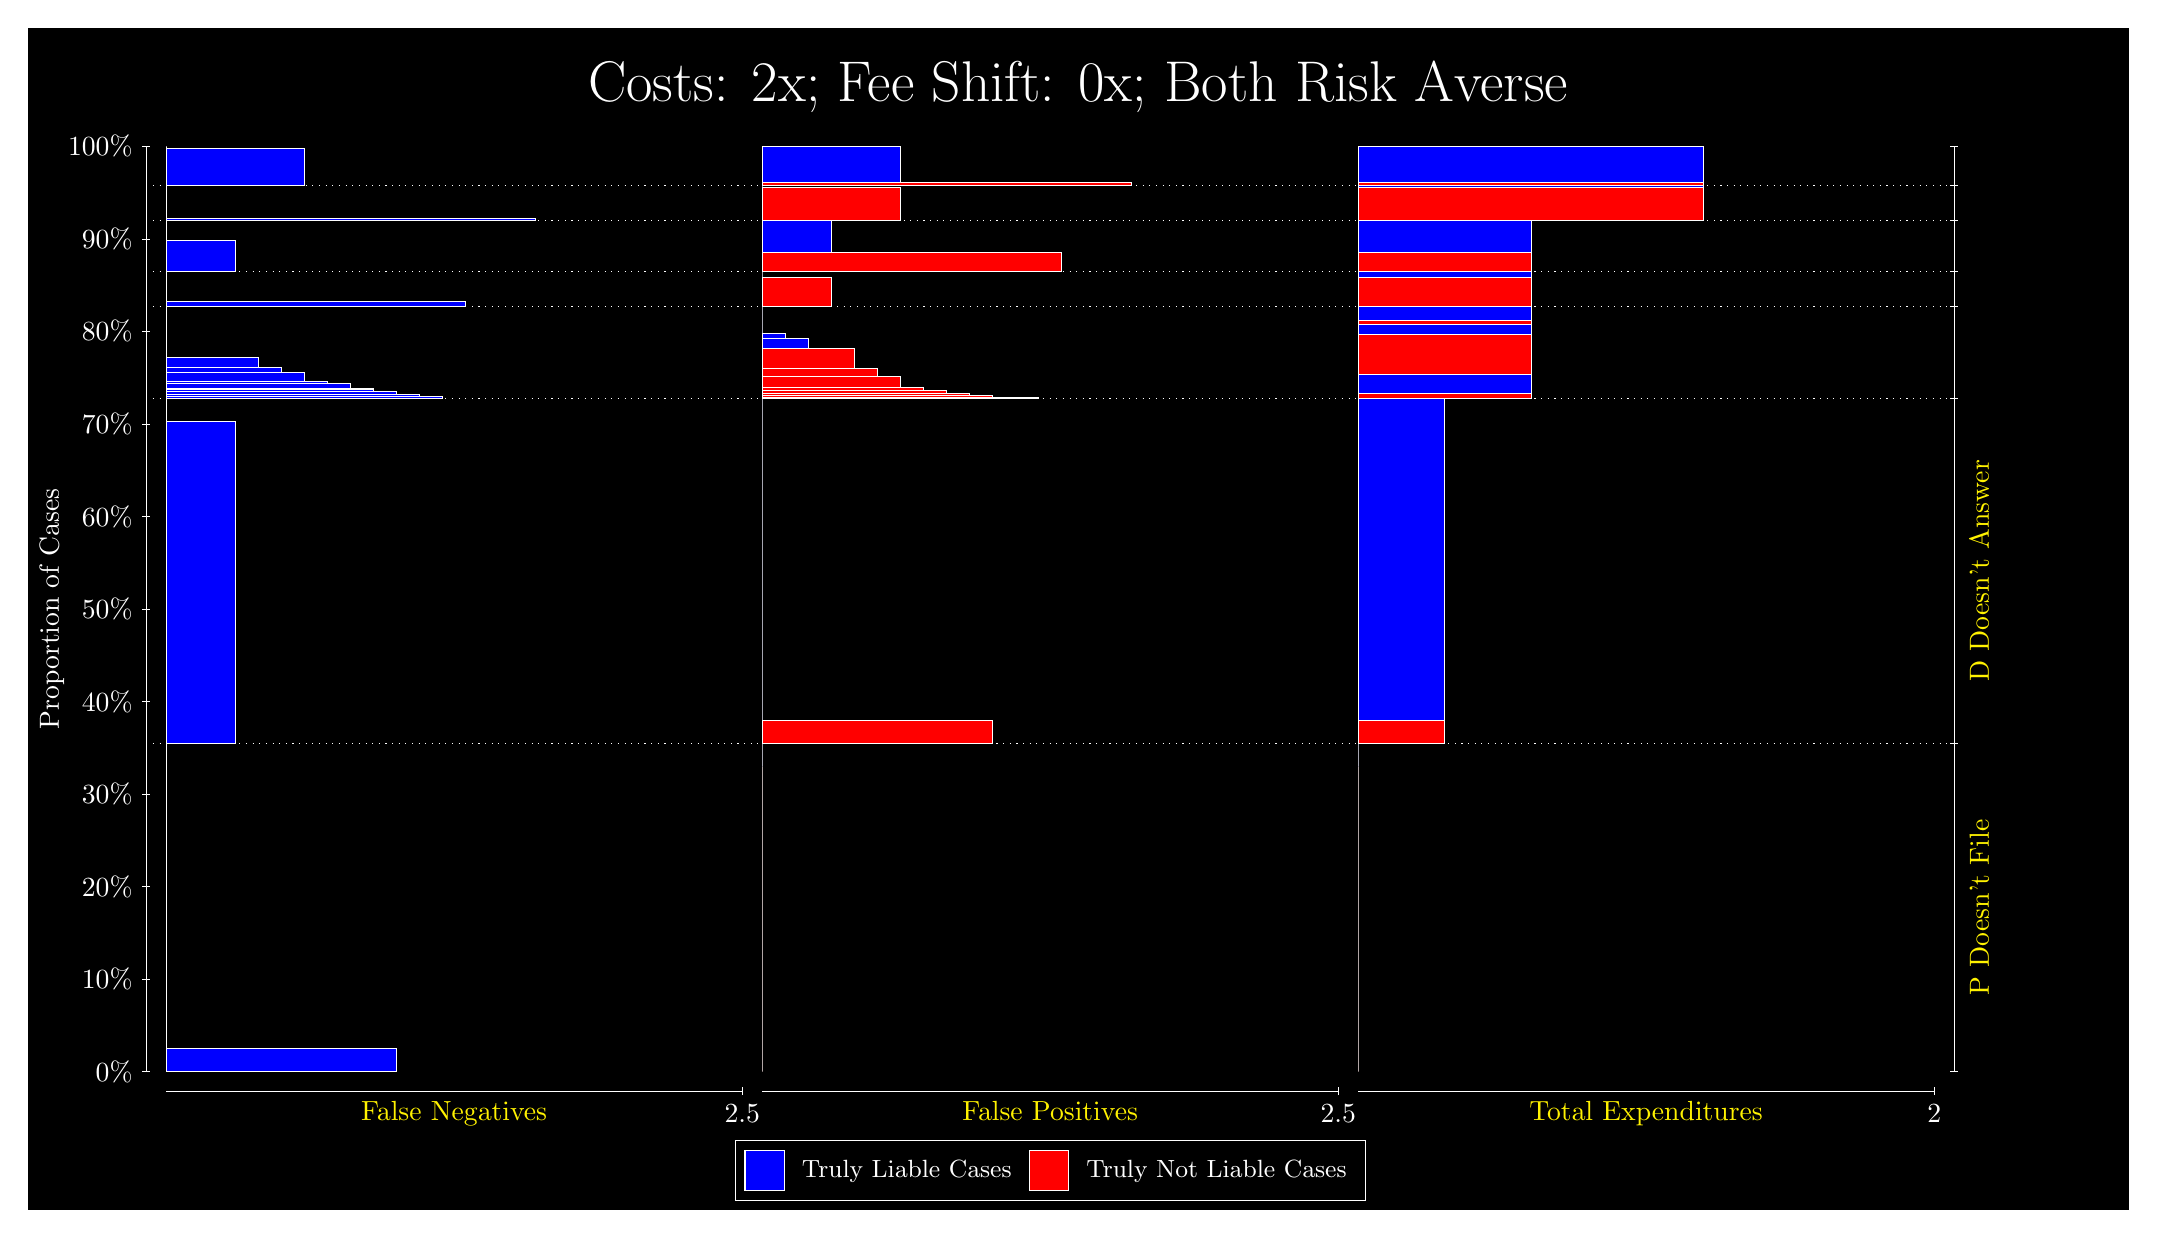
\begin{tikzpicture}
\draw[fill=black] (0,0) rectangle (26.667,15);
\draw[text=white] (0,13.5) rectangle (26.667,15) node[midway] {\huge Costs: 2x; Fee Shift: 0x; Both Risk Averse};
\draw[white, very thin] (1.5,1.75) -- (1.5,13.5);
\node[rotate=90, text=white, anchor=center] at (0.3, 7.625) {Proportion of Cases};
\draw[white, very thin] (1.45,1.75) -- (1.55,1.75);
\node[text=white, anchor=east] at (1.45, 1.75) {0\%};
\draw[white, very thin] (1.45,2.925) -- (1.55,2.925);
\node[text=white, anchor=east] at (1.45, 2.925) {10\%};
\draw[white, very thin] (1.45,4.1) -- (1.55,4.1);
\node[text=white, anchor=east] at (1.45, 4.1) {20\%};
\draw[white, very thin] (1.45,5.275) -- (1.55,5.275);
\node[text=white, anchor=east] at (1.45, 5.275) {30\%};
\draw[white, very thin] (1.45,6.45) -- (1.55,6.45);
\node[text=white, anchor=east] at (1.45, 6.45) {40\%};
\draw[white, very thin] (1.45,7.625) -- (1.55,7.625);
\node[text=white, anchor=east] at (1.45, 7.625) {50\%};
\draw[white, very thin] (1.45,8.8) -- (1.55,8.8);
\node[text=white, anchor=east] at (1.45, 8.8) {60\%};
\draw[white, very thin] (1.45,9.975) -- (1.55,9.975);
\node[text=white, anchor=east] at (1.45, 9.975) {70\%};
\draw[white, very thin] (1.45,11.15) -- (1.55,11.15);
\node[text=white, anchor=east] at (1.45, 11.15) {80\%};
\draw[white, very thin] (1.45,12.325) -- (1.55,12.325);
\node[text=white, anchor=east] at (1.45, 12.325) {90\%};
\draw[white, very thin] (1.45,13.5) -- (1.55,13.5);
\node[text=white, anchor=east] at (1.45, 13.5) {100\%};

\draw[white, very thin] (24.457,1.75) -- (24.457,13.5);
\draw[white, very thin] (24.407,1.75) -- (24.507,1.75);
\node[anchor=west] at (24.407, 1.75) {};
\draw[white, very thin] (24.407,5.9206) -- (24.507,5.9206);
\node[anchor=west] at (24.407, 5.9206) {};
\draw[white, very thin] (24.407,10.299) -- (24.507,10.299);
\node[anchor=west] at (24.407, 10.299) {};
\draw[white, very thin] (24.407,11.463) -- (24.507,11.463);
\node[anchor=west] at (24.407, 11.463) {};
\draw[white, very thin] (24.407,11.909) -- (24.507,11.909);
\node[anchor=west] at (24.407, 11.909) {};
\draw[white, very thin] (24.407,12.556) -- (24.507,12.556);
\node[anchor=west] at (24.407, 12.556) {};
\draw[white, very thin] (24.407,13.007) -- (24.507,13.007);
\node[anchor=west] at (24.407, 13.007) {};
\draw[white, very thin] (24.407,13.5) -- (24.507,13.5);
\node[anchor=west] at (24.407, 13.5) {};

\draw[white, very thin, fill=blue] (1.75,1.75) rectangle (4.6775,2.0493);
\draw[white, very thin, fill=red] (1.75,2.0493) rectangle (1.75,5.9206);
\draw[white, very thin, fill=blue] (1.75,5.9206) rectangle (2.6283,10.008);
\draw[white, very thin, fill=red] (1.75,10.008) rectangle (1.75,10.299);
\draw[white, very thin, fill=blue] (1.75,10.299) rectangle (5.2631,10.325);
\draw[white, very thin, fill=blue] (1.75,10.325) rectangle (4.9703,10.35);
\draw[white, very thin, fill=blue] (1.75,10.35) rectangle (4.6775,10.388);
\draw[white, very thin, fill=blue] (1.75,10.388) rectangle (4.3848,10.418);
\draw[white, very thin, fill=blue] (1.75,10.418) rectangle (4.3848,10.433);
\draw[white, very thin, fill=blue] (1.75,10.433) rectangle (4.092,10.485);
\draw[white, very thin, fill=blue] (1.75,10.485) rectangle (3.7993,10.517);
\draw[white, very thin, fill=blue] (1.75,10.517) rectangle (3.5065,10.636);
\draw[white, very thin, fill=blue] (1.75,10.636) rectangle (3.2138,10.697);
\draw[white, very thin, fill=blue] (1.75,10.697) rectangle (2.921,10.826);
\draw[white, very thin, fill=red] (1.75,10.826) rectangle (1.75,11.463);
\draw[white, very thin, fill=blue] (1.75,11.463) rectangle (5.5558,11.532);
\draw[white, very thin, fill=red] (1.75,11.532) rectangle (1.75,11.909);
\draw[white, very thin, fill=blue] (1.75,11.909) rectangle (2.6283,12.306);
\draw[white, very thin, fill=red] (1.75,12.306) rectangle (1.75,12.556);
\draw[white, very thin, fill=blue] (1.75,12.556) rectangle (6.4341,12.589);
\draw[white, very thin, fill=red] (1.75,12.589) rectangle (1.75,13.007);
\draw[white, very thin, fill=blue] (1.75,13.007) rectangle (3.5065,13.469);
\draw[white, very thin, fill=red] (1.75,13.469) rectangle (1.75,13.5);
\draw[white, very thin, fill=red] (9.3189,1.75) rectangle (9.3189,5.6213);
\draw[white, very thin, fill=blue] (9.3189,5.6213) rectangle (9.3189,5.9206);
\draw[white, very thin, fill=red] (9.3189,5.9206) rectangle (12.246,6.2118);
\draw[white, very thin, fill=blue] (9.3189,6.2118) rectangle (9.3189,10.299);
\draw[white, very thin, fill=red] (9.3189,10.299) rectangle (12.832,10.308);
\draw[white, very thin, fill=red] (9.3189,10.308) rectangle (12.539,10.318);
\draw[white, very thin, fill=red] (9.3189,10.318) rectangle (12.246,10.338);
\draw[white, very thin, fill=red] (9.3189,10.338) rectangle (11.954,10.363);
\draw[white, very thin, fill=red] (9.3189,10.363) rectangle (11.661,10.402);
\draw[white, very thin, fill=red] (9.3189,10.402) rectangle (11.368,10.434);
\draw[white, very thin, fill=red] (9.3189,10.434) rectangle (11.075,10.575);
\draw[white, very thin, fill=red] (9.3189,10.575) rectangle (10.783,10.683);
\draw[white, very thin, fill=red] (9.3189,10.683) rectangle (10.49,10.935);
\draw[white, very thin, fill=blue] (9.3189,10.935) rectangle (9.9044,11.065);
\draw[white, very thin, fill=blue] (9.3189,11.065) rectangle (9.6116,11.126);
\draw[white, very thin, fill=blue] (9.3189,11.126) rectangle (9.3189,11.463);
\draw[white, very thin, fill=red] (9.3189,11.463) rectangle (10.197,11.84);
\draw[white, very thin, fill=blue] (9.3189,11.84) rectangle (9.3189,11.909);
\draw[white, very thin, fill=red] (9.3189,11.909) rectangle (13.125,12.16);
\draw[white, very thin, fill=blue] (9.3189,12.16) rectangle (10.197,12.556);
\draw[white, very thin, fill=red] (9.3189,12.556) rectangle (11.075,12.974);
\draw[white, very thin, fill=blue] (9.3189,12.974) rectangle (9.3189,13.007);
\draw[white, very thin, fill=red] (9.3189,13.007) rectangle (14.003,13.038);
\draw[white, very thin, fill=blue] (9.3189,13.038) rectangle (11.075,13.5);
\draw[white, very thin, fill=red] (16.888,1.75) rectangle (16.888,5.6213);
\draw[white, very thin, fill=blue] (16.888,5.6213) rectangle (16.888,5.9206);
\draw[white, very thin, fill=red] (16.888,5.9206) rectangle (17.986,6.2118);
\draw[white, very thin, fill=blue] (16.888,6.2118) rectangle (17.986,10.299);
\draw[white, very thin, fill=red] (16.888,10.299) rectangle (19.083,10.369);
\draw[white, very thin, fill=blue] (16.888,10.369) rectangle (19.083,10.601);
\draw[white, very thin, fill=red] (16.888,10.601) rectangle (19.083,11.119);
\draw[white, very thin, fill=blue] (16.888,11.119) rectangle (19.083,11.239);
\draw[white, very thin, fill=red] (16.888,11.239) rectangle (19.083,11.287);
\draw[white, very thin, fill=blue] (16.888,11.287) rectangle (19.083,11.463);
\draw[white, very thin, fill=red] (16.888,11.463) rectangle (19.083,11.84);
\draw[white, very thin, fill=blue] (16.888,11.84) rectangle (19.083,11.909);
\draw[white, very thin, fill=red] (16.888,11.909) rectangle (19.083,12.16);
\draw[white, very thin, fill=blue] (16.888,12.16) rectangle (19.083,12.556);
\draw[white, very thin, fill=red] (16.888,12.556) rectangle (21.279,12.974);
\draw[white, very thin, fill=blue] (16.888,12.974) rectangle (21.279,13.007);
\draw[white, very thin, fill=red] (16.888,13.007) rectangle (21.279,13.038);
\draw[white, very thin, fill=blue] (16.888,13.038) rectangle (21.279,13.5);
\draw[white, dotted] (1.5,5.9206) -- (24.457,5.9206);
\draw[white, dotted] (1.5,10.299) -- (24.457,10.299);
\draw[white, dotted] (1.5,11.463) -- (24.457,11.463);
\draw[white, dotted] (1.5,11.909) -- (24.457,11.909);
\draw[white, dotted] (1.5,12.556) -- (24.457,12.556);
\draw[white, dotted] (1.5,13.007) -- (24.457,13.007);
\draw[white, very thin] (1.75,1.5) -- (9.0689,1.5);
\node[text=yellow, anchor=north] at (5.4094, 1.5) {False Negatives};
\draw[white, very thin] (9.0689,1.45) -- (9.0689,1.55);
\node[text=white, anchor=north] at (9.0689, 1.45) {2.5};

\draw[white, very thin] (9.3189,1.5) -- (16.638,1.5);
\node[text=yellow, anchor=north] at (12.978, 1.5) {False Positives};
\draw[white, very thin] (16.638,1.45) -- (16.638,1.55);
\node[text=white, anchor=north] at (16.638, 1.45) {2.5};

\draw[white, very thin] (16.888,1.5) -- (24.207,1.5);
\node[text=yellow, anchor=north] at (20.547, 1.5) {Total Expenditures};
\draw[white, very thin] (24.207,1.45) -- (24.207,1.55);
\node[text=white, anchor=north] at (24.207, 1.45) {2};

\node[text=yellow, centered, rotate=90] at (24.777, 3.8353) {P Doesn't File};
\node[text=yellow, centered, rotate=90] at (24.777, 8.1097) {D Doesn't Answer};






\draw (12.978300999999998,1.5) node[draw=none] (baseCoordinate) {};
\begin{scope}[align=center]
        \matrix[scale=0.5, draw=white, below=0.5cm of baseCoordinate, nodes={draw}, column sep=0.1cm]{
            \node[rectangle, draw, minimum width=0.5cm, minimum height=0.5cm, fill=blue] {}; &
            \node[draw=none, font=\small, text=white] (B) {Truly Liable Cases}; &
            \node[rectangle, draw, minimum width=0.5cm, minimum height=0.5cm, fill=red] {}; &
            \node[draw=none, font=\small, text=white] (B) {Truly Not Liable Cases}; \\
            };
\end{scope}

\end{tikzpicture}
\end{document}